\renewcommand{\theequation}{\theenumi}
\begin{enumerate}[label=\thesubsection.\arabic*.,ref=\thesubsection.\theenumi]
\numberwithin{equation}{enumi}
%
\item Solve
\label{prob:lp_std}
\begin{align}
\max_{\vec{x}} Z &= \myvec{4 & 1}\vec{x}
\\
s.t. \quad 
\myvec{
1 & 1
\\
3 & 1
}
\vec{x} &\preceq \myvec{50\\90}
\\
\vec{x} &\succeq \vec{0}
\end{align}
%
using cvxpy.
\\
\solution The given problem can be expressed in general as
\begin{align}
\max_{\vec{x}} &\vec{c}^{T}\vec{x}
\\
s.t. \quad \vec{A}\vec{x} &\le \vec{b},
\\
\vec{x} &\succeq\vec{0}
\end{align}
%
where
\begin{align}
\vec{c} &= \myvec{4 \\ 1}
\\
\vec{A} &=
\myvec{
1 & 1
\\
3 & 1
}
\\
\vec{b}&=\myvec{50\\90}
%
\end{align}
%
and can be solved using {\em cvxpy} through the following code
\begin{lstlisting}
codes/opt/lp_cvx.py
\end{lstlisting}
%
to obtain
\begin{align}
\vec{x} = \myvec{30\\0}, Z = 120
\end{align}
%
\item Graphically, show that the {feasible region} in  Problem \ref{prob:lp_std} result in the interior of a convex polygon and the optimal point is one of the vertices.
\solution The following code plots Fig. \ref{fig:lp_feas_reg}.
%
\begin{lstlisting}
codes/opt/lp_cvx.py
\end{lstlisting}
%
\begin{figure}[!ht]
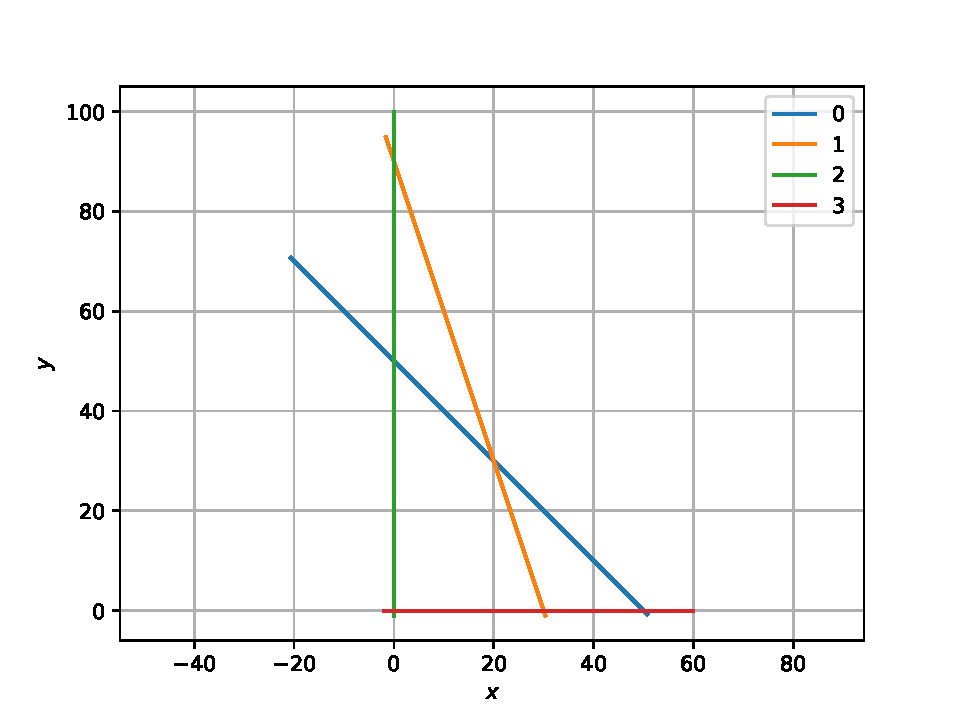
\includegraphics[width=\columnwidth]{./figs/opt/lp_feas_reg.eps}
\caption{}
\label{fig:lp_feas_reg}
\end{figure}

%Verify the solution to graphically.
\item Solve
\begin{align}
\min_{\vec{x}} Z &= \myvec{3 & 9}\vec{x}
\\
s.t. \quad 
\myvec{
1 & 3
\\
-1 & -1
\\
1 & -1
}
\vec{x} &\preceq \myvec{60\\-10\\0}
\\
\vec{x} &\succeq \vec{0}
\label{eq:lp_exam_mult}
\end{align}
\solution The following code
\begin{lstlisting}
codes/opt/lp_cvx_mult.py
\end{lstlisting}
%
is used to obtain
\begin{align}
\vec{x} = \myvec{15\\15}, Z = 180
\end{align}
%
%\item Write a program to plot the constraints for any linear program.

%The region in \eqref{eq:lp_constr} is shown in Fig. \ref{}
\item Solve
\begin{align}
\min_{\vec{x}} Z &= \myvec{-50 & 20}\vec{x}
\\
s.t. \quad 
\myvec{
-2 & 1
\\
-3 & -1
\\
2 & -3
}
\vec{x} &\preceq \myvec{5\\-3\\12}
\\
\vec{x} &\succeq \vec{0}
\end{align}
%
\solution The following code 
\begin{lstlisting}
codes/opt/lp_cvx_nosol.py
\end{lstlisting}
%
shows that the given problem has no solution.
\item Verify all the above solutions using Lagrange multipliers.
\item Repeat the above exercise using the Simplex method.
\item\textbf {(Diet problem)}: A dietician wishes to mix two types of foods in such a
way that vitamin contents of the mixture contain atleast 8 units of vitamin A and 10
units of vitamin C. Food ‘I’ contains 2 units/kg of vitamin A and 1 unit/kg of vitamin C.
Food ‘II’ contains 1 unit/kg of vitamin A and 2 units/kg of vitamin C. It costs
Rs 50 per kg to purchase Food ‘I’ and Rs 70 per kg to purchase Food ‘II’. Formulate
this problem as a linear programming problem to minimise the cost of such a mixture.
\\
\solution Let the mixture contain $x$ kg of food I and $y$ kg of food II.
\\
\begin{table}[!h]
\begin{tabular}{|l|l|l|l|}
\hline
\multirow{2}{*}{Resources} & \multicolumn{2}{l|}{Food} & \multirow{2}{*}{Requirement} \\ \cline{2-3}
                           & I           & II          &                              \\ \hline
Vitamin A                  & 2           & 1           & Atleast 8 Units              \\ \hline
Vitamin C                  & 1           & 2           & Atleast 10 Units             \\ \hline
Cost                       & 50          & 70          &                              \\ \hline
\end{tabular}
\end{table}
%
The given problem can be expressed as
%GOAL: We need to minimize the cost of mixture.\\
%Cost of FOOD I per kg = Rs 50 \\
%Cost of FOOD II per kg = Rs 70 \\
% Minimize $ Z = 50x +70y$\\
% Subject to constraints:\\
% $2x+y>=8$\\
% $x+2y>=10$\\
% $x,y>=0$\\
\begin{align}
\min_{\vec{x}} Z &= \myvec{50 & 70}\vec{x}
\\
s.t. \quad 
\myvec{
2 & 1
\\
1 & 2
%\\
%2 & -3
}
\vec{x} & \succeq \myvec{8\\10}
%\preceq \myvec{5\\-3\\12}
\\
\vec{x} &\succeq \vec{0}
\label{eq:diet}
\end{align}
%
The corner points of the feasible region are available in Table \ref{table:diet_corner_pt} and plotted in Fig. \ref{fig:diet}.
%
\begin{table}[!h]
\begin{tabular}{|l|l|l|l|}
\hline
Corner Point &  $Z=50x+70y$\\
\hline
(0,8)& 560\\
\hline
(2,4)& 380\\
\hline
(10,0)& 500\\
\hline
\end{tabular}
\caption{}
\label{table:diet_corner_pt}
\end{table}
  \begin{figure}[!h]

  \centering
  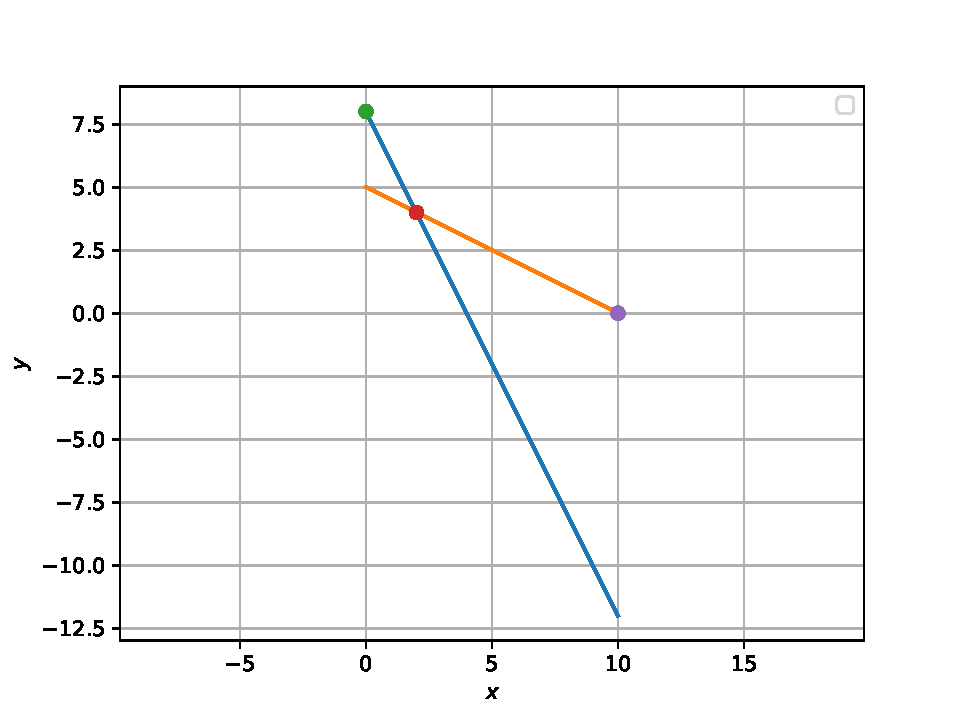
\includegraphics[width=1\linewidth]{./figs/opt/lp_diet.eps}
\caption{}
\label{fig:diet}
  \end{figure}


The smallest value of Z is 380 at the point (2,4). But the feasible region is unbounded therefore we draw the graph of the inequality
\begin{align}
50x +70y<380
\end{align}
to check whether the resulting open half has any point common with the feasible region but on checking it doesn't have any points in common. 
Thus the minimum value of Z is 380 attained at $\myvec{2\\4}$. Hence optimal mixing strategy for the dietician would be to mix 2 Kg of Food I and 4 Kg of Food II.  The following code provides the solution to \eqref{eq:diet}.
%
\begin{lstlisting}
codes/opt/diet.py
\end{lstlisting}



\item \textbf{(Allocation problem)} A cooperative society of farmers has 50 hectare
of land to grow two crops X and Y. The profit from crops X and Y per hectare are
estimated as Rs 10,500 and Rs 9,000 respectively. To control weeds, a liquid herbicide
has to be used for crops X and Y at rates of 20 litres and 10 litres per hectare. Further,
no more than 800 litres of herbicide should be used in order to protect fish and wild life
using a pond which collects drainage from this land. How much land should be allocated
to each crop so as to maximise the total profit of the society?\\
\solution The given problem can be formulated as
\begin{align}
\max_{\vec{x}} Z &= \myvec{10500 & 9000}\vec{x}
\\
s.t. \quad 
\myvec{
20 & 10
}
\vec{x} & \preceq 800
\\
\myvec{
1 & 1
} 
\vec{x} &= 50
\label{eq:allocation}
\end{align}
Fig  \ref{fig:allocation}
shows the intersection of various lines and the optimal point as indicated.
\begin{figure}[h]
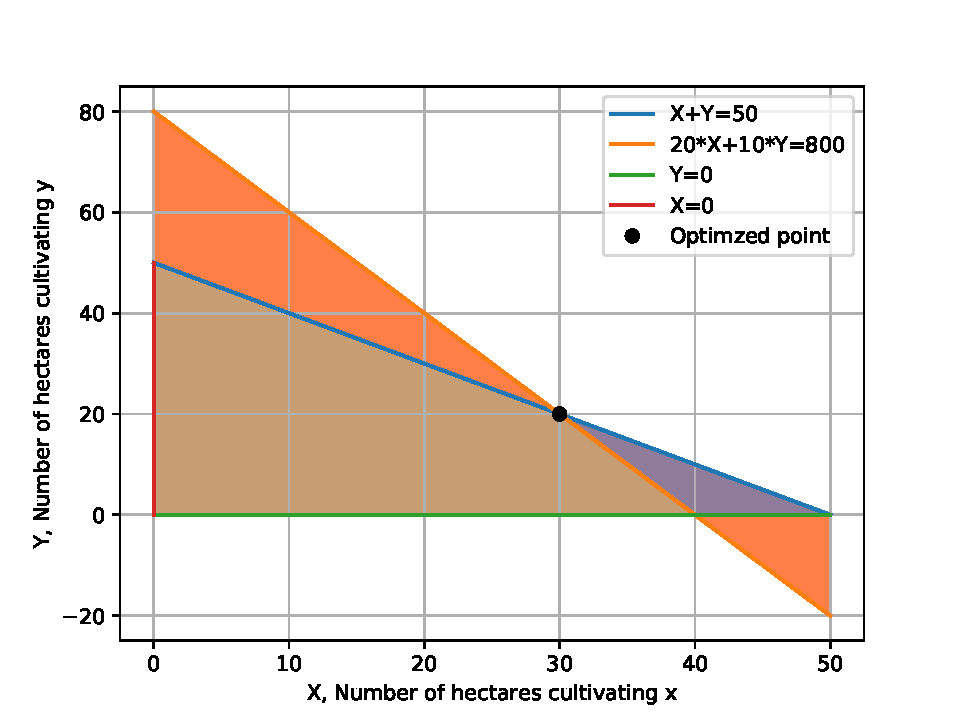
\includegraphics[width=\columnwidth]{./figs/opt/lp_allocation.eps}
\caption{Feasible region for allocation Problem}
\caption{}
\label{fig:allocation}
\end{figure}

The following code provides the solution to \eqref{eq:allocation} at \myvec{30\\20}.
%
\begin{lstlisting}
codes/opt/allocation.py
\end{lstlisting}

\item \textbf{(Manufacturing problem)} A manufacturer has three machines I, II
and III installed in his factory. Machines I and II are capable of being operated for
at most 12 hours whereas machine III must be operated for atleast 5 hours a day. She
produces only two items M and N each requiring the use of all the three machines.
The number of hours required for producing 1 unit of each of M and N on the three
machines are given in the following table:\\

\begin{tabular}{|c|c|c|c|}
\hline
 \multicolumn{3}{|l}{\textbf{ Number of hours required on machines}}& \\ \cline{2-4}
\hline
\textbf {Items}&\textbf{I}&\textbf{II}&\textbf{III}\\
\hline
M&1&2&1\\
\hline
 N&2&1&1.25\\
 \hline 

\end{tabular}

She makes a profit of Rs 600 and Rs 400 on items M and N respectively. How many
of each item should she produce so as to maximise her profit assuming that she can sell
all the items that she produced? What will be the maximum profit?
\\
\solution The given problem can be formulated as
\begin{align}
\max_{\vec{x}} Z &= \myvec{80000&12000}\vec{x}
\\
s.t. \quad 
\myvec{
3 & 4
\\
1 & 3
}
\vec{x} & \preceq \myvec{60\\30}
\label{eq:manufacturing}
\end{align}

Fig  \ref{fig:manufacturing}
shows the intersection of various lines and the optimal point as indicated.
\begin{figure}[h]
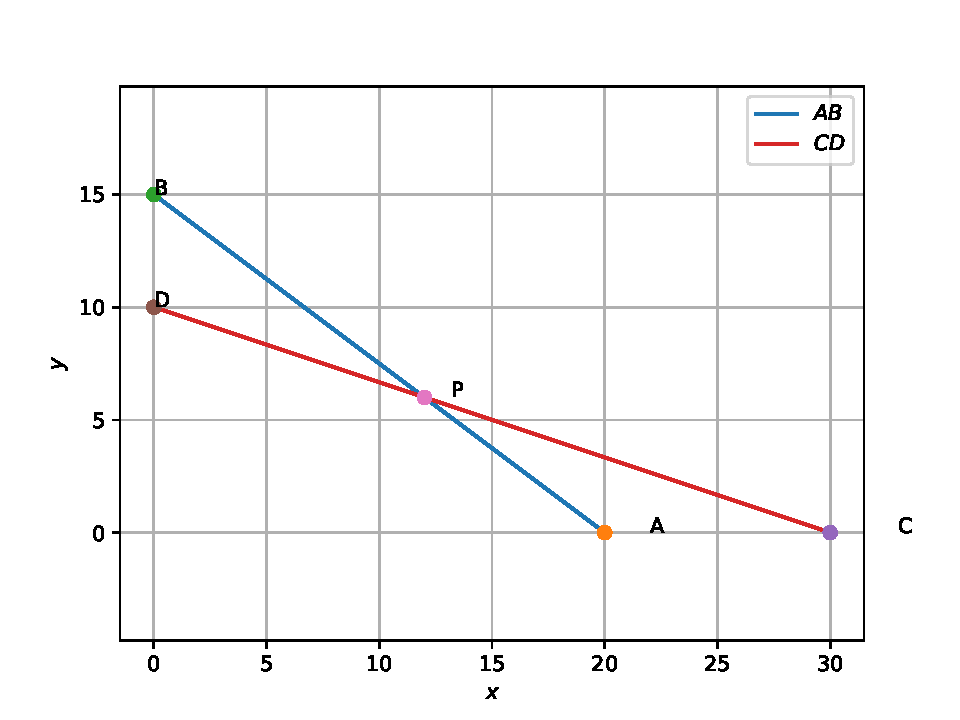
\includegraphics[width=\columnwidth]{./figs/opt/lp_manufacturing.eps}
\caption{Feasible region for manufacturing Problem}
\caption{}
\label{fig:manufacturing}
\end{figure}

The following code provides the solution to \eqref{eq:manufacturing} at \myvec{12\\6}.
%
\begin{lstlisting}
codes/opt/Manufacturing.py
\end{lstlisting}

\item \textbf{(Transportation problem)} There are two factories located one at
place P and the other at place Q. From these locations, a certain commodity is to be
delivered to each of the three depots situated at A, B and C. The weekly requirements
of the depots are respectively 5, 5 and 4 units of the commodity while the production
capacity of the factories at P and Q are respectively 8 and 6 units. The cost of transportation per unit is given below where A,B,C are cost in ruppes:\\
\begin{tabular}{|c|c|c|c|}
\hline
From/To & A & B & C\\
\hline
P & 160 & 100 & 150\\
\hline
Q & 100 &120 & 100\\
\hline
\end{tabular}\\
How many units should be transported from each factory to each depot in order that
the transportation cost is minimum. What will be the minimum transportation cost?
\\
\solution The given problem can be formulated as
\begin{align}
\min_{\vec{x}} Z &= \myvec{10 & -70}\vec{x}
\\
s.t. \quad 
\myvec{
1 & 1
\\
-1 & -1
}
\vec{x} & \preceq \myvec{8\\-4}
\\
\vec{x} &\preceq \myvec{5\\5}
\label{eq:transport}
\end{align}

Fig  \ref{fig:transport}
shows the intersection of various lines and the optimal point indicated as OPT PT.
\begin{figure}[h]
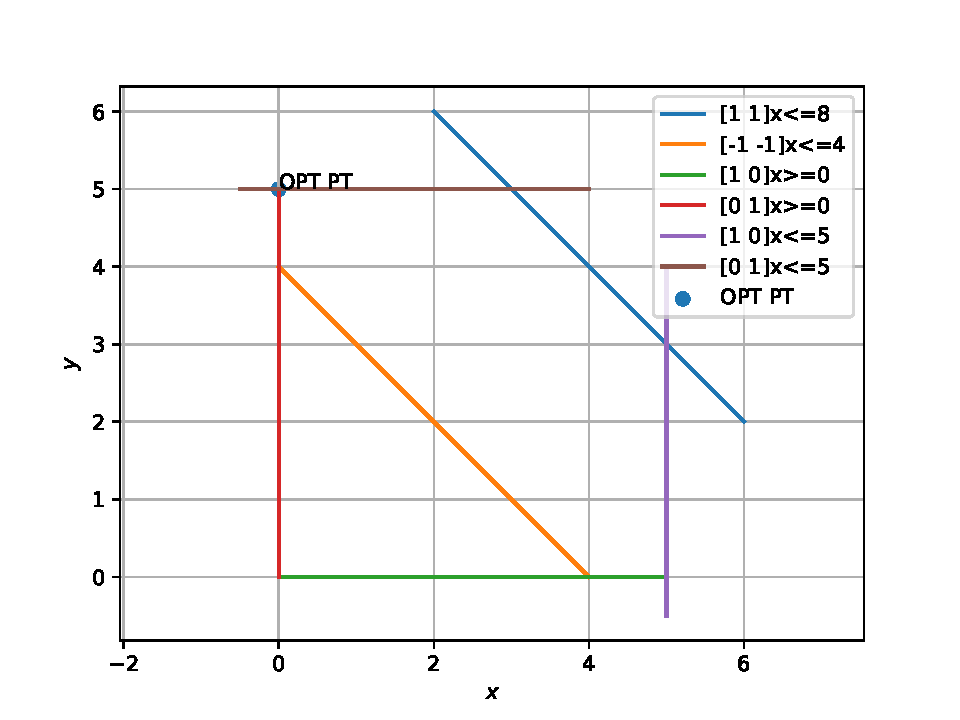
\includegraphics[width=\columnwidth]{./figs/opt/lp_transport.eps}
\caption{Feasible region for Transportation Problem}
\caption{}
\label{fig:transport}
\end{figure}

The following code provides the solution to \eqref{eq:transport} at \myvec{0\\5}.
%
\begin{lstlisting}
codes/opt/Transportation.py
\end{lstlisting}





\end{enumerate}
%    \end{document}
    
